\documentclass[landscape]{article}
\usepackage{graphicx,color,amssymb}
%% \usepackage{bm}
\pagestyle{empty}
\oddsidemargin  -0.5 in
\evensidemargin -0.5 in
\headheight     0 in
\topmargin      -1 in
\textheight     7.7 in
\textwidth      10 in
\newenvironment{slide}[1][ ]{\mbox{\bf #1 } \vfill}{\vfill \mbox{ } \pagebreak}
\begin{document}
\huge
\renewcommand{\labelitemi}{-}
\setlength{\parindent}{0 cm}

\begin{slide}
  \begin{center}
    
\includegraphics[height=3 cm]{title}

    \vspace{2 cm}
    \Huge Jim Pivarski
  \end{center}
\end{slide}

\begin{slide}[Method]
  Use production process $e^+e^- \to \Upsilon$, integrated over $e^+e^-$ energy

  \vfill
  \[\Gamma_{ee} = \frac{{M_\Upsilon}^2}{6\pi^2} \int \sigma(e^+e^- \to \Upsilon) \, dE, \]

  \vfill
  Integral will be replaced by a fit to production lineshape, excluding ISR tail

  \vfill
  \begin{center}
    \includegraphics[width=0.6\linewidth]{../proceedings_cartoon}    
  \end{center}

  \vfill
  Lineshape scans were acquired in November 2001 -- September 2002

\end{slide}

\begin{slide}[Method]
  Measure cross-section by counting hadrons, correct for leptons with $(1-3\mathcal{B}_{\mu\mu})$

  \vfill
  \begin{center}
    \begin{tabular}{p{0.33\linewidth} p{0.65\linewidth}}
      \begin{minipage}{\linewidth}
	Hadron cuts:
	\renewcommand{\labelenumi}{(\alph{enumi})}
	\begin{enumerate}
	  \item largest track momentum \\ $<$ 70\% beam energy
	  \item visible energy $>$ 40\% of \\ center-of-mass energy
	  \item event vertex XY within \\ 5 mm of beamspot
	  \item event vertex Z within \\ 7.5 cm of beamspot
	\end{enumerate}
      \end{minipage} &
      \begin{minipage}{\linewidth}
	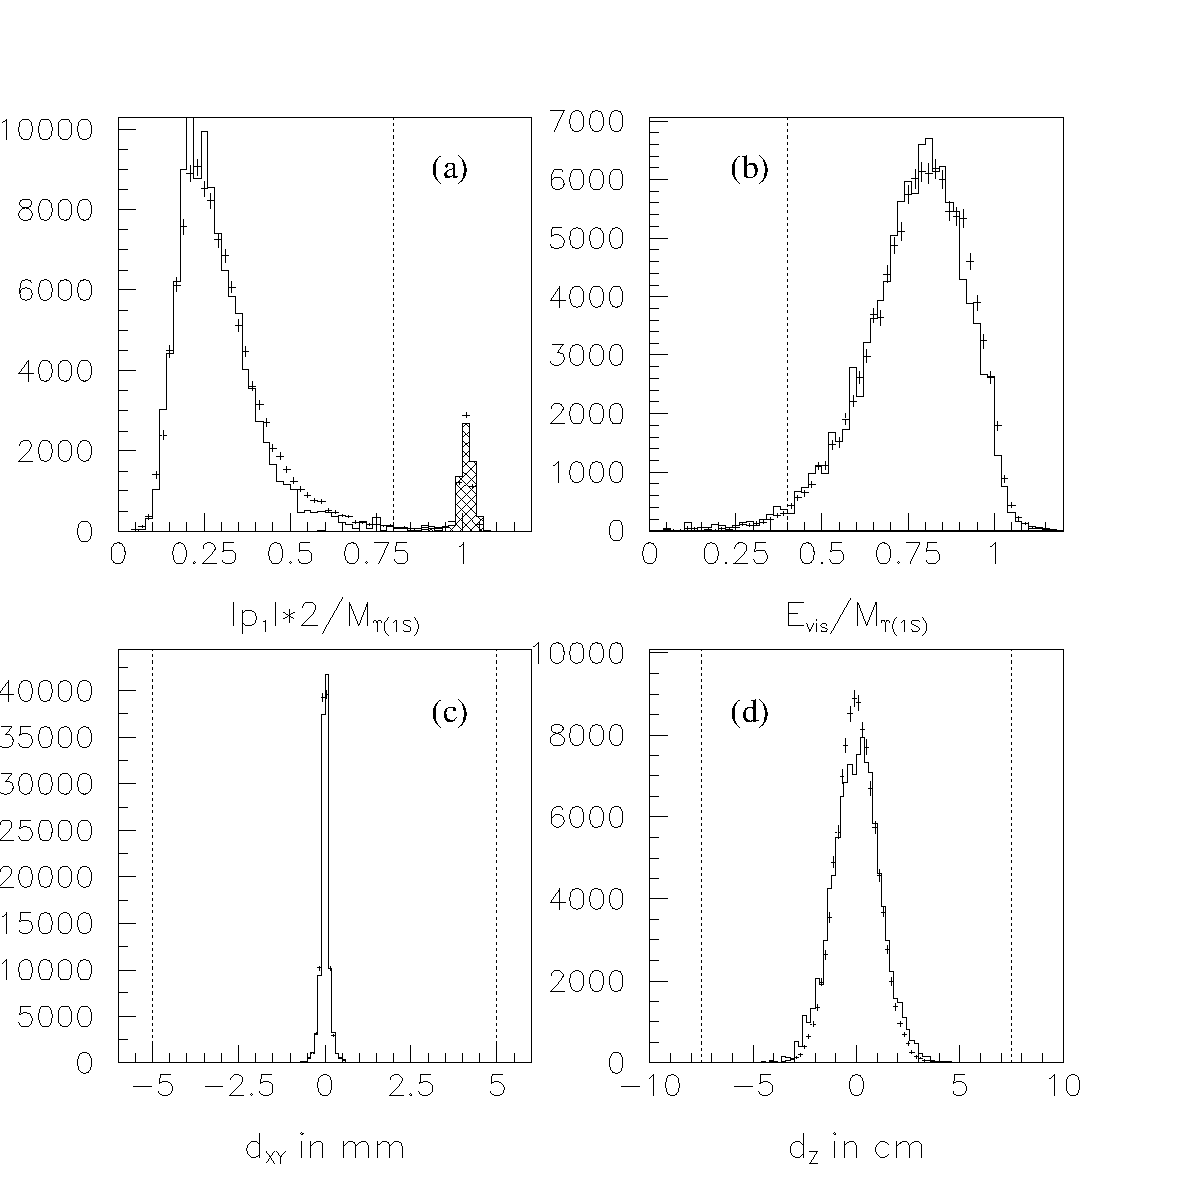
\includegraphics[width=\linewidth, bb=0 0 540 520]{../proceedings_cuts3}
      \end{minipage}
    \end{tabular}
  \end{center}
\end{slide}

\begin{slide}[Issues (Table of Contents):]
  \Huge

  \vspace{-3 cm}
  \begin{center}
    \begin{minipage}{19 cm}
      \begin{itemize}\setlength{\itemsep}{0.5 cm}
	\item {\bf Hadronic efficiency}
        \item {\bf Backgrounds}
	\item {\bf Luminosity}
	\item {\bf Cross-section stability}
	\item {\bf Beam-energy measurement stability}
        \item {\bf Fitting}
      \end{itemize}
    \end{minipage}
  \end{center}

  \vspace{1.5 cm}
  {\bf \huge And then}
  \begin{center}
    \begin{minipage}{19 cm}

      \begin{itemize}\setlength{\itemsep}{0.5 cm}
        \item {\bf Preliminary results}
      \end{itemize}
    \end{minipage}
  \end{center}
\end{slide}

\begin{slide}[Hadronic Efficiency]

  \vspace{-1.5 cm}
  \begin{center}
    \begin{tabular}{p{0.63\linewidth} p{0.35\linewidth}}
      \begin{minipage}{\linewidth}
	$\Upsilon(1S)$ measured directly in $\Upsilon(2S) \to \pi^+\pi^- \Upsilon(1S)$

	\vspace{0.5 cm}
	\mbox{\hspace{0.25 cm}} {\large $\bullet$} $\pi^+\pi^-$ chosen to satisfy trigger

	\vspace{0.5 cm}
	\mbox{\hspace{0.25 cm}} {\large $\bullet$} Corrected for boost, track/shower confusion

	\vspace{0.5 cm}
	Hadronic efficiency is (97.8 $\pm$ 0.5)\%
      \end{minipage} &
      \begin{minipage}{\linewidth}
	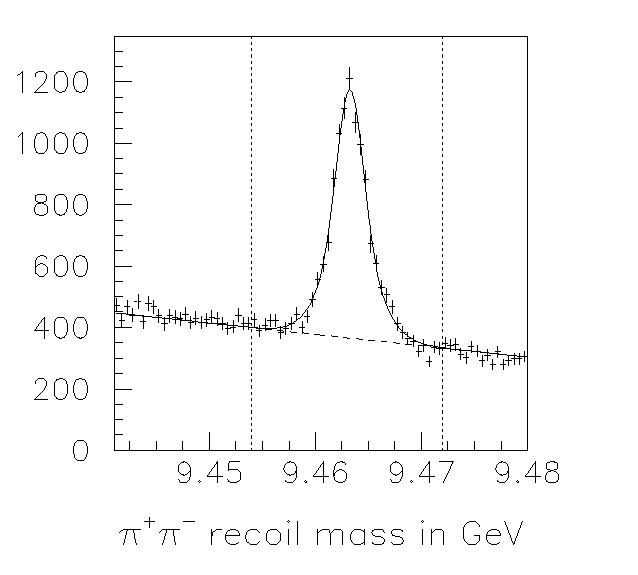
\includegraphics[width=\linewidth]{../plenary_justpipimass}
      \end{minipage}
    \end{tabular}
  \end{center}

  \textcolor{white}{Correct $\Upsilon(2,3S)$ for cascades to leptons}

  \vspace{0.1 cm}
  \begin{center}
    \begin{tabular}{p{0.45\linewidth} p{0.45\linewidth}}
      \begin{minipage}{\linewidth}
	\begin{center}
	  \textcolor{white}{$\mathcal{B}_{X\ell^+\ell^-}$ = (1.5 $\pm$ 0.4)\%}

	  \vspace{0.1 cm}
	  \includegraphics[width=0.7\linewidth]{../cascade_correction_white}
	\end{center}
      \end{minipage} &
      \begin{minipage}{\linewidth}
	\begin{center}
	  \textcolor{white}{$\mathcal{B}_{X\ell^+\ell^-}$ = (1.4 $\pm$ 0.5)\%}

	  \vspace{0.1 cm}
	  \includegraphics[width=0.7\linewidth]{../cascade_correction_white}
	\end{center}
      \end{minipage}
    \end{tabular}
  \end{center}

  \vspace{0.1 cm}
  \textcolor{white}{Hadronic efficiency is (96.1 $\pm$ 0.6)\% (2S) and (96.2 $\pm$ 0.7)\% (3S)}
\end{slide}

\begin{slide}[Hadronic Efficiency]

  \vspace{-1.5 cm}
  \begin{center}
    \begin{tabular}{p{0.63\linewidth} p{0.35\linewidth}}
      \begin{minipage}{\linewidth}
	$\Upsilon(1S)$ measured directly in $\Upsilon(2S) \to \pi^+\pi^- \Upsilon(1S)$

	\vspace{0.5 cm}
	\mbox{\hspace{0.25 cm}} {\large $\bullet$} $\pi^+\pi^-$ chosen to satisfy trigger

	\vspace{0.5 cm}
	\mbox{\hspace{0.25 cm}} {\large $\bullet$} Corrected for boost, track/shower confusion

	\vspace{0.5 cm}
	Hadronic efficiency is (97.8 $\pm$ 0.5)\%
      \end{minipage} &
      \begin{minipage}{\linewidth}
	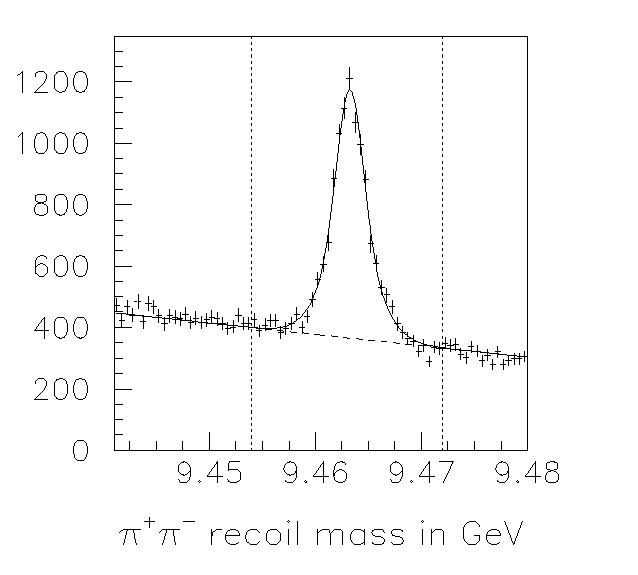
\includegraphics[width=\linewidth]{../plenary_justpipimass}
      \end{minipage}
    \end{tabular}
  \end{center}

  Correct $\Upsilon(2,3S)$ for cascades to leptons

  \vspace{0.1 cm}
  \begin{center}
    \begin{tabular}{p{0.45\linewidth} p{0.45\linewidth}}
      \begin{minipage}{\linewidth}
	\begin{center}
	  $\mathcal{B}_{X\ell^+\ell^-}$ = (1.5 $\pm$ 0.4)\%

	  \vspace{0.1 cm}
	  \includegraphics[width=0.7\linewidth]{../cascade_correction_2s}
	\end{center}
      \end{minipage} &
      \begin{minipage}{\linewidth}
	\begin{center}
	  $\mathcal{B}_{X\ell^+\ell^-}$ = (1.4 $\pm$ 0.5)\% 

	  \vspace{0.1 cm}
	  \includegraphics[width=0.7\linewidth]{../cascade_correction_3s}
	\end{center}
      \end{minipage}
    \end{tabular}
  \end{center}

  \vspace{0.1 cm}
  Hadronic efficiency is (96.1 $\pm$ 0.6)\% (2S) and (96.2 $\pm$ 0.7)\% (3S)
\end{slide}

\begin{slide}[Backgrounds]
  Explicitly subtract cosmic rays and beam-gas, effectively subtract the rest in the fit

  \vspace{0.6 cm}
  \begin{center}
    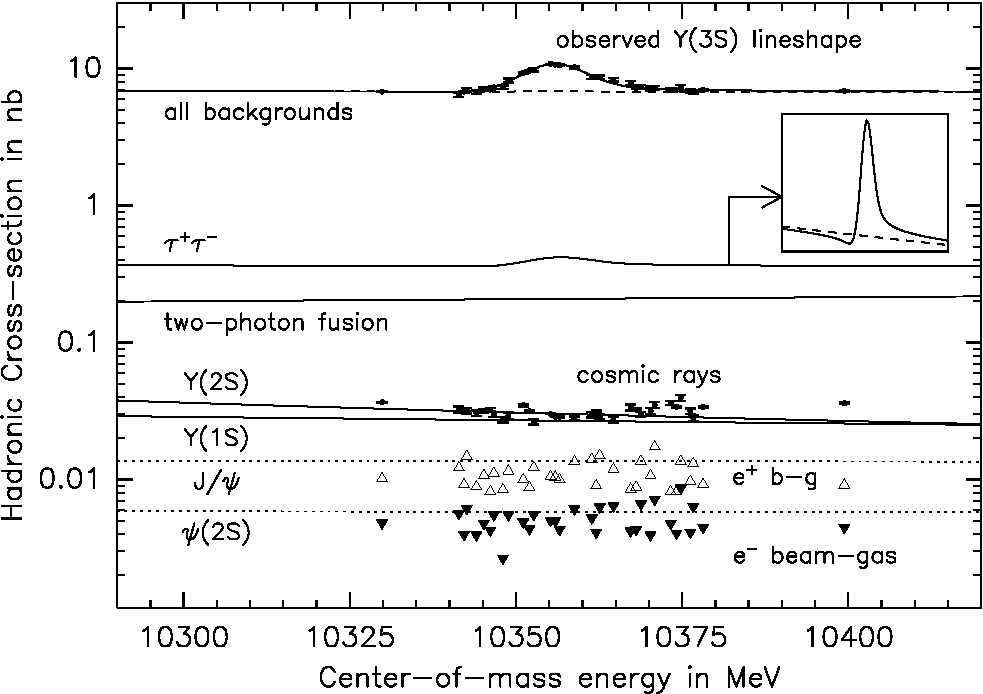
\includegraphics[width=0.9\linewidth]{../jed_backgrounds}
  \end{center}

  \vspace{-1 cm}
\end{slide}

\begin{slide}[Luminosity]

  \vfill
  Surik and Brian determined luminosity calibration to 1.3\% (CBX 05-17)

  \vfill
  \begin{center}
    \Huge All off-resonance data \\
    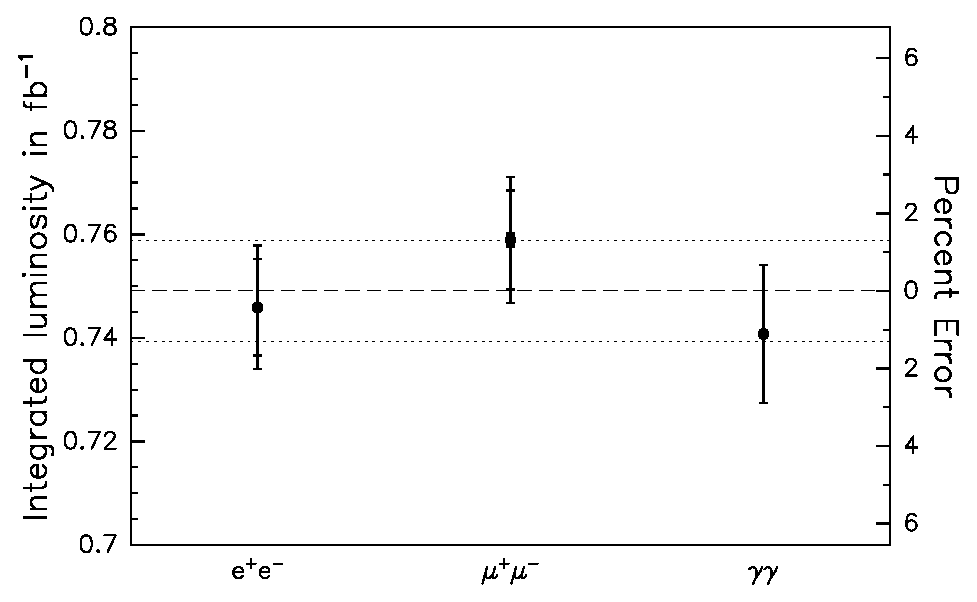
\includegraphics[width=0.75\linewidth]{../plenary_lumi}
  \end{center}

  \vfill
  We use $\gamma\gamma$ for point-by-point luminosity (no backgrounds
  from $\Upsilon$), and the above average to normalize all luminosities
\end{slide}

\begin{slide}[Cross-section Stability]
  \Huge
  All off-resonance runs at a given energy reproduce the same cross-section, within statistics

  \vfill
  \begin{center}
    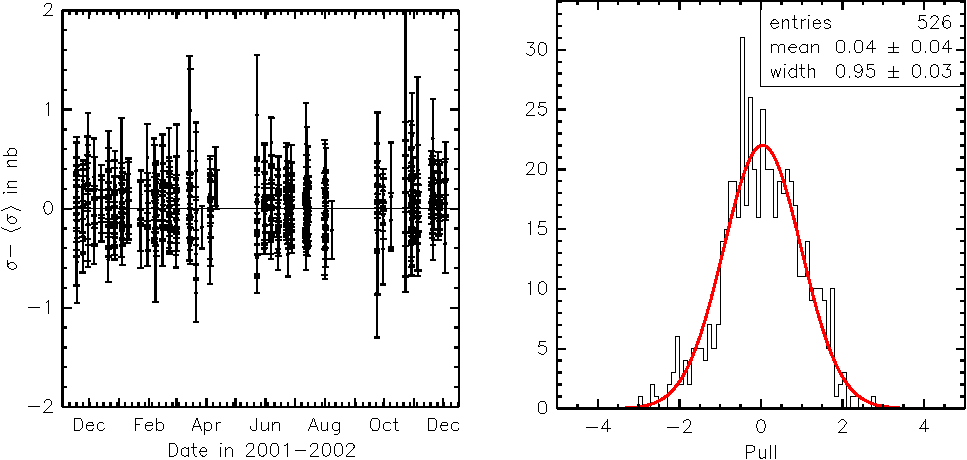
\includegraphics[width=\linewidth]{stability}
  \end{center}

  \vfill
  Cross-section {\bf in}stability $\lesssim$ 0.03 nb
\end{slide}

\begin{slide}[Beam-energy Measurement Stability]
  \begin{tabular}{p{0.6\linewidth} p{0.38\linewidth}}
    \begin{minipage}{\linewidth}
      \begin{itemize}
	\item weekly scans were short and \\ independent
	\item measurements alternated above and \\ below resonance peak
	\item a point of high slope was repeated \\ in the scan
      \end{itemize}

      \vspace{0.5 cm}
      \begin{center}
	
\includegraphics[width=0.95\linewidth]{../proceedings_miscal_white}

	\vspace{1 cm}
	\textcolor{white}{Beam-energy {\bf in}stability $\lesssim$ 0.07 MeV}
      \end{center}

    \end{minipage} &
    \begin{minipage}{\linewidth}
      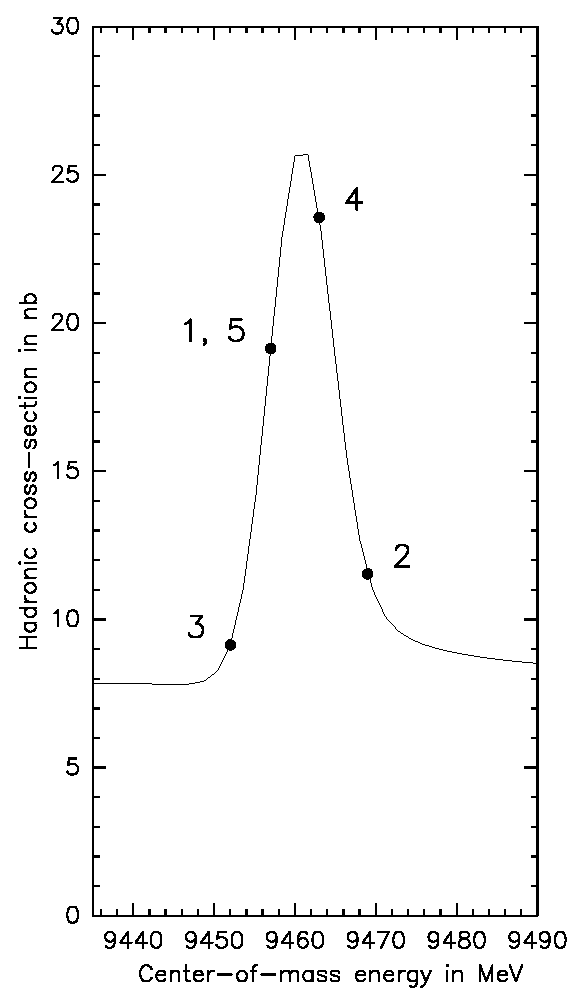
\includegraphics[width=\linewidth]{../plenary_fitorder}
    \end{minipage}
  \end{tabular}
\end{slide}

\begin{slide}[Beam-energy Measurement Stability]
  \begin{tabular}{p{0.6\linewidth} p{0.38\linewidth}}
    \begin{minipage}{\linewidth}
      \begin{itemize}
	\item weekly scans were short and \\ independent
	\item measurements alternated above and \\ below resonance peak
	\item a point of high slope was repeated \\ in the scan
      \end{itemize}

      \vspace{0.5 cm}
      \begin{center}
	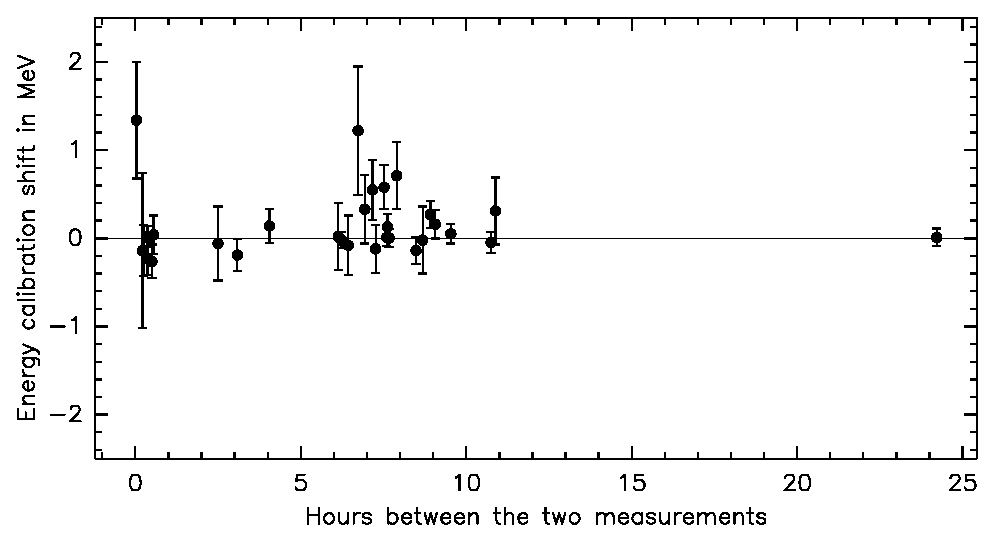
\includegraphics[width=0.95\linewidth]{../proceedings_miscal}

	\vspace{1 cm}
	Beam-energy {\bf in}stability $\lesssim$ 0.07 MeV
      \end{center}

    \end{minipage} &
    \begin{minipage}{\linewidth}
      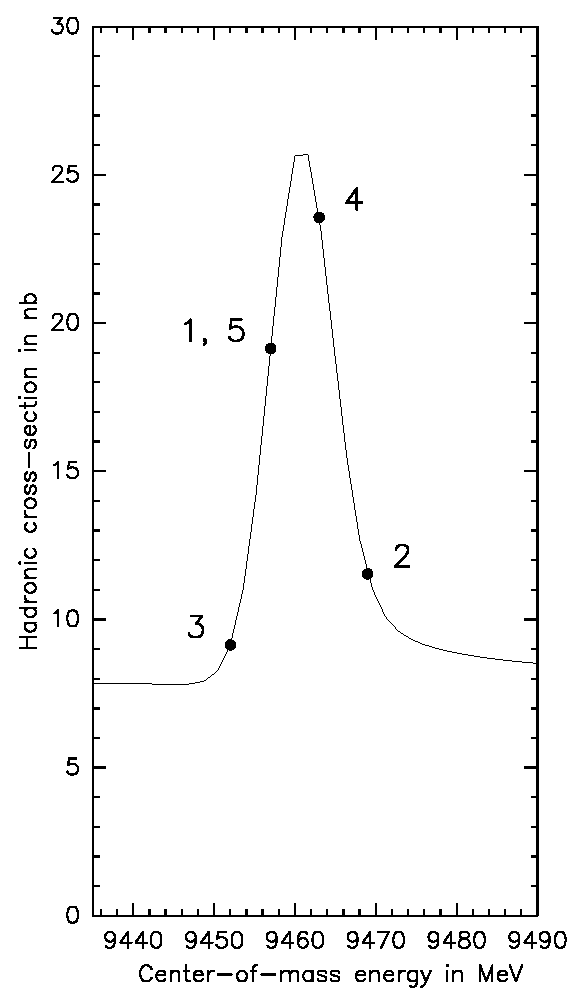
\includegraphics[width=\linewidth]{../plenary_fitorder}
    \end{minipage}
  \end{tabular}
\end{slide}

\begin{slide}[Fitting]
  \begin{tabular}{p{0.6\linewidth} p{0.38\linewidth}}
    \begin{minipage}{\linewidth}
      {\bf Parameters:}

      \vspace{0.75 cm}
      \mbox{\hspace{1 cm}} \begin{minipage}{0.85\linewidth}
	\begin{enumerate}\setlength{\itemsep}{0.5 cm}
	  \item Area without tail (MeV nb) $\longrightarrow$ $\Gamma_{ee}$ (keV)
	  \item Beam energy spread (MeV)
	  \item Background level (nb)
	    \renewcommand{\labelenumi}{4--15.}
	  \item Upsilon mass for each weekly scan (MeV)
	\end{enumerate}
      \end{minipage}

      \vspace{1 cm}
      {\bf Fit function:}

      \vspace{0.75 cm}
      \mbox{\hspace{1 cm}} \begin{minipage}{0.85\linewidth}
	\begin{enumerate}\setlength{\itemsep}{0.75 cm}
	  \item Breit-Wigner $\otimes$ Gaussian $\otimes$ ISR tail \\
	    (Kuraev and Fadin 0.1\% calculation)
	    
	    Includes interference term (small effect)
	  \item $\tau^+\tau^-$ background peaks under signal, \\
	    precisely subtracted with Jean's $\mathcal{B}_{\tau\tau}$
	  \item Smooth backgrounds: $1/s$ and $\log s$
	\end{enumerate}
      \end{minipage}
    \end{minipage} &
    \begin{minipage}{\linewidth}
      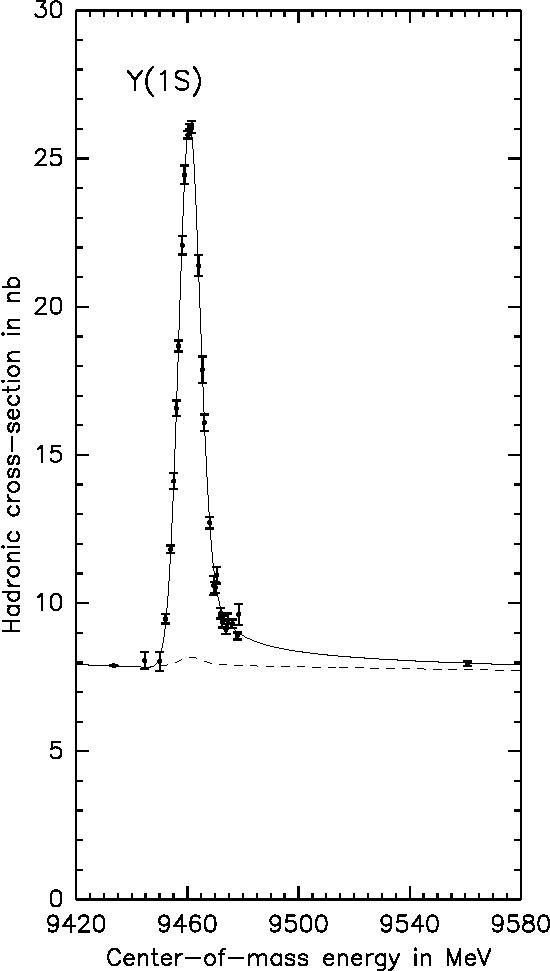
\includegraphics[width=\linewidth]{../individual_noinset_1s}
    \end{minipage}
  \end{tabular}
\end{slide}

\begin{slide}[Fit Results]

  \vspace{0.6 cm}
  \begin{center}
    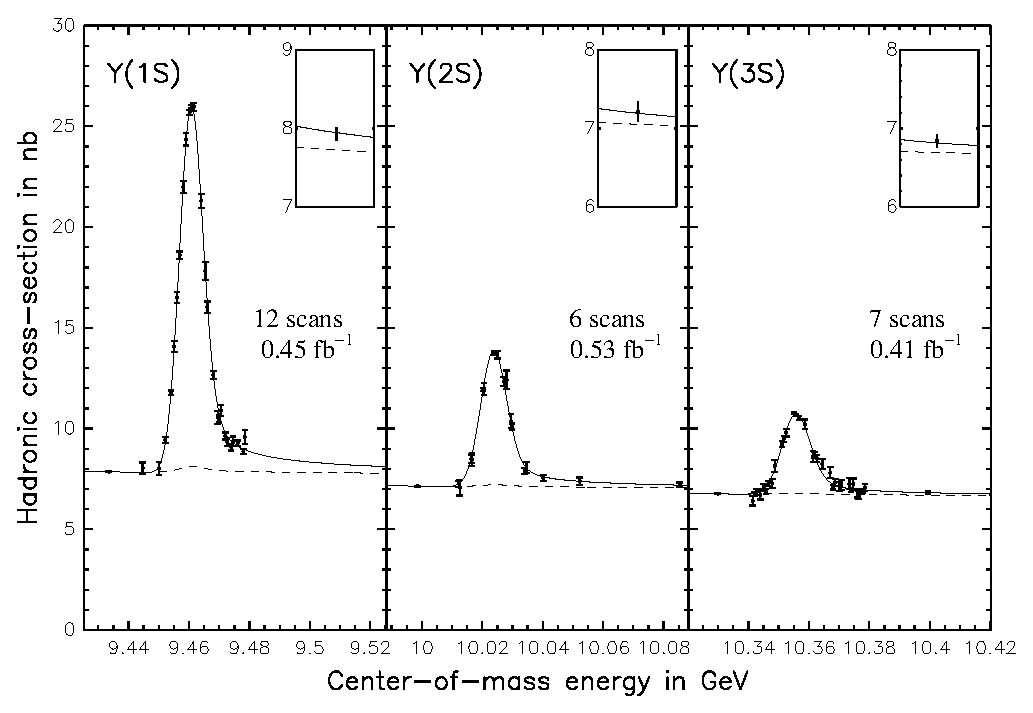
\includegraphics[width=\linewidth]{../three_resonances_inset_squat2_nscans}
  \end{center}

  \vspace{-0.6 cm}
\end{slide}

\begin{slide}[$\bf \Upsilon(1S)$ Pull Distributions: $\bf \chi^2/$ndf = 230/195 = 1.2, C.L. = 4\%]
  \begin{center}
    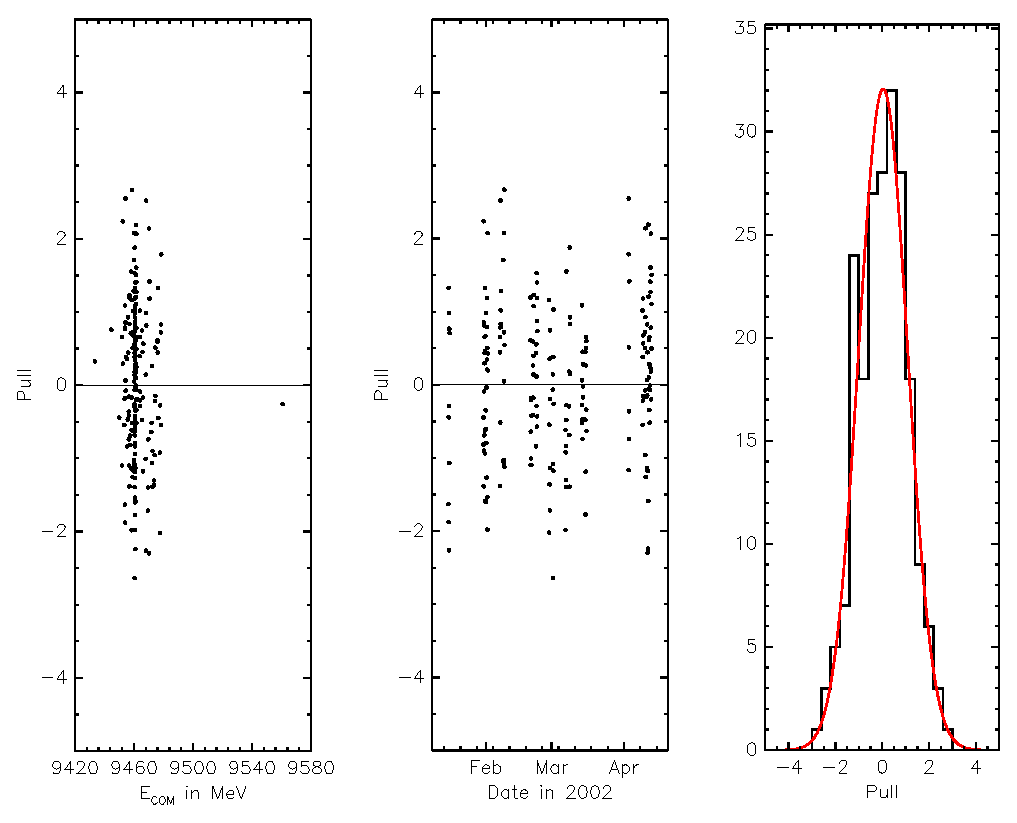
\includegraphics[width=0.85\linewidth]{../plenary_pulls1}
  \end{center}
\end{slide}

\begin{slide}[$\bf \Upsilon(2S)$ Pull Distributions: $\bf \chi^2/$ndf = 58/66 = 0.87, C.L. = 76\%]
  \begin{center}
    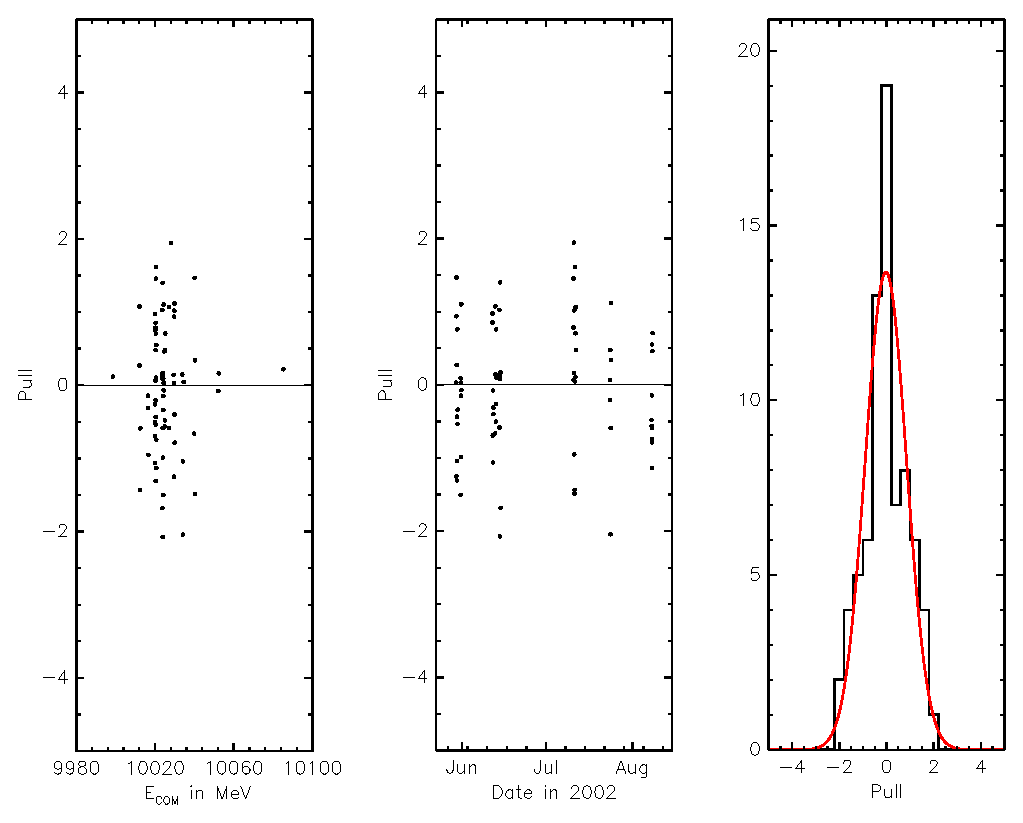
\includegraphics[width=0.85\linewidth]{../plenary_pulls2}
  \end{center}
\end{slide}

\begin{slide}[$\bf \Upsilon(3S)$ Pull Distributions: $\bf \chi^2/$ndf = 155/165 = 0.94, C.L. = 70\%]
  \begin{center}
    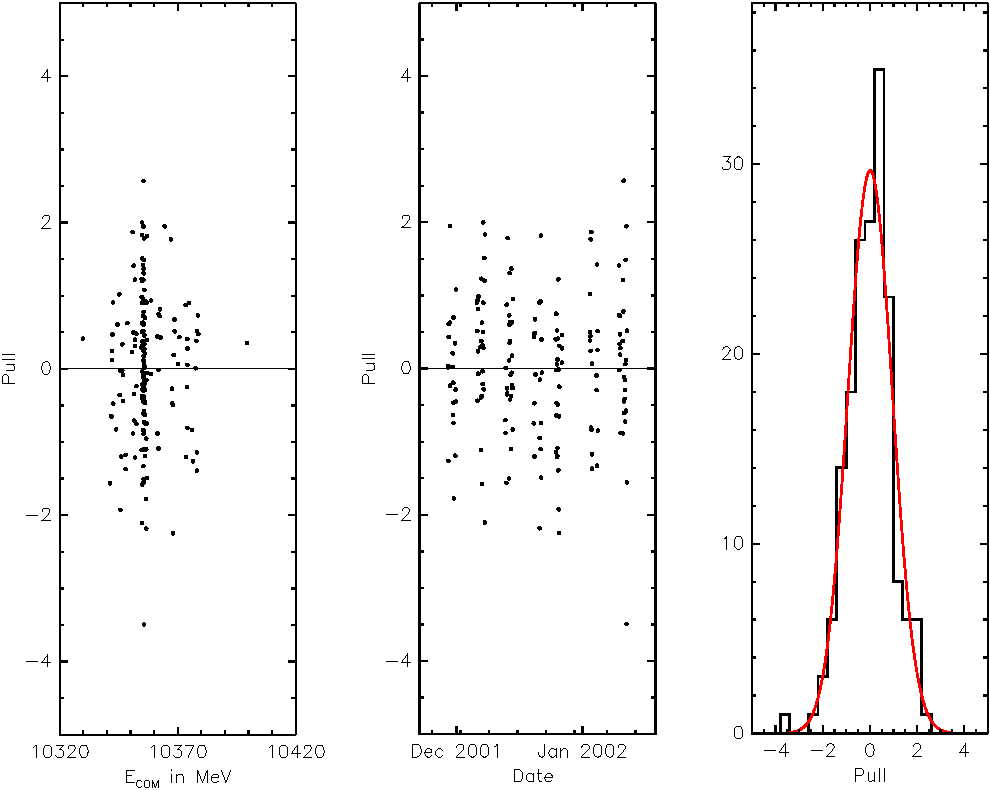
\includegraphics[width=0.85\linewidth]{../plenary_pulls3}
  \end{center}
\end{slide}

%% \begin{slide}
%%   \begin{center}
%%     \begin{tabular}{l c c c}
%%       \hline\hline
%%       Contribution to $\Gamma_{ee}$ & $\Upsilon(1S)$ & $\Upsilon(2S)$ & $\Upsilon(3S)$ \\\hline
%%       Statistical$^*$               & 0.7\%  & 1.6\%  & 2.2\% \\
%%       Hadronic efficiency           & 0.5\%  & 0.6\%  & 0.7\% \\
%%       $(1 - 3\mathcal{B}_{\mu\mu})$ & 0.2\%  & 0.2\%  & 0.3\% \\
%%       Luminosity calibration        & 1.3\%  & 1.3\%  & 1.3\% \\
%%       Shape of the fit function     & 0.05\% & 0.06\% & 0.05\% \\
%%       Cross-section stability       & 0.1\%  & 0.1\%  & 0.1\% \\
%%       Beam-energy stability         & 0.2\%  & 0.2\%  & 0.2\% \\\hline
%%       Result (in keV $\pm$ {\it stat} $\pm$ {\it syst}) & & \mbox{\hspace{-3 cm}} 0.616 $\pm$ 0.010 $\pm$ 0.009 \mbox{\hspace{-3 cm}} & \\ 
%%       & \mbox{\hspace{-0.3 cm}} 1.336 $\pm$ 0.009 $\pm$ 0.019 \mbox{\hspace{-0.3 cm}} & & \mbox{\hspace{-0.3 cm}} 0.425 $\pm$ 0.009 $\pm$ 0.006 \mbox{\hspace{-0.3 cm}} \\
%%       Fractional uncertainty        & 1.6\%  & 2.2\%  & 2.7\% \\\hline\hline    
%%       & & & \\
%%       \hline\hline
%%       Ratios of $\Gamma_{ee}$             & 2S/1S & 3S/1S & 3S/2S \\\hline
%%       Result (in keV $\pm$ {\it stat} $\pm$ {\it syst}) & & \mbox{\hspace{-3 cm}} 0.318 $\pm$ 0.007 $\pm$ 0.002 \mbox{\hspace{-3 cm}} & \\ 
%%       & \mbox{\hspace{-0.3 cm}} 0.461 $\pm$ 0.008 $\pm$ 0.003 \mbox{\hspace{-0.3 cm}} & & \mbox{\hspace{-0.3 cm}} 0.690 $\pm$ 0.019 $\pm$ 0.006 \mbox{\hspace{-0.3 cm}} \\
%%       Fractional uncertainty        & 1.8\%  & 2.4\%  & 2.8\% \\\hline\hline    
%%     \end{tabular}
%%   \end{center}

%%   \vspace{1 cm}
%%   $^*$ \begin{minipage}{0.9\linewidth}

%%     \vspace{0.6 cm}
%%     Statistical uncertainty is dominated by run-by-run luminosity
%%     measurement ($e^+e^- \to \gamma\gamma$ counting) and contains
%%     background subtractions.
%%   \end{minipage}
%% \end{slide}

\begin{slide}[Summary of Uncertainties]
  \begin{center}
    \renewcommand{\arraystretch}{1.25}
    \begin{tabular}{l c c c}
      Contribution to $\Gamma_{ee}$ & \mbox{\hspace{1 cm}} $\Upsilon(1S)$ \mbox{\hspace{1 cm}} & \mbox{\hspace{1 cm}} $\Upsilon(2S)$ \mbox{\hspace{1 cm}} & \mbox{\hspace{1 cm}} $\Upsilon(3S)$ \mbox{\hspace{1 cm}} \\\hline
      Statistical$^*$               & {\bf 0.7\%}  & {\bf 1.6\%}  & {\bf 2.2\%} \\
      $(1 - 3\mathcal{B}_{\mu\mu})$ & 0.2\%  & 0.2\%  & 0.3\% \\
      Hadronic efficiency           & 0.5\%  & 0.6\%  & 0.7\% \\
      Luminosity calibration        & {\bf 1.3\%}  & {\bf 1.3\%}  & {\bf 1.3\%} \\
      Cross-section stability       & 0.1\%  & 0.1\%  & 0.1\% \\
      Beam-energy stability         & 0.2\%  & 0.2\%  & 0.2\% \\
      Shape of the fit function     & 0.05\% & 0.06\% & 0.05\% \\\hline
      Total                         & {\bf 1.6\%}  & {\bf 2.2\%}  & {\bf 2.7\%} \\
    \end{tabular}
  \end{center}

  \vspace{1 cm}
  \mbox{ }$^*$\begin{minipage}{0.9\linewidth}

    \vspace{1 cm}
    Statistical uncertainty is dominated by run-by-run luminosity
    measurement ($e^+e^- \to \gamma\gamma$ counting) and contains
    background subtractions.
  \end{minipage}
\end{slide}

\begin{slide}[Preliminary Results]
  \begin{center}
    \renewcommand{\arraystretch}{2}
    \begin{tabular}{c c c}
      Quantity & Value & \mbox{\hspace{0.5 cm}} Uncertainty \mbox{\hspace{0.5 cm}} \\ \hline
      $\Gamma_{ee}(1S)$ & \mbox{\hspace{0.5 cm}} 1.336 $\pm$ 0.009 $\pm$ 0.019 keV \mbox{\hspace{0.5 cm}} & 1.6\% \\
      $\Gamma_{ee}(2S)$ & 0.616 $\pm$ 0.010 $\pm$ 0.009 keV & 2.2\% \\
      $\Gamma_{ee}(3S)$ & 0.425 $\pm$ 0.009 $\pm$ 0.006 keV & 2.7\% \\ \hline
      $\Gamma_{ee}(2S)$/$\Gamma_{ee}(1S)$ & 0.461 $\pm$ 0.008 $\pm$ 0.003 & 1.8\% \\
      $\Gamma_{ee}(3S)$/$\Gamma_{ee}(1S)$ & 0.318 $\pm$ 0.007 $\pm$ 0.002 & 2.4\% \\
      $\Gamma_{ee}(3S)$/$\Gamma_{ee}(2S)$ & 0.690 $\pm$ 0.019 $\pm$ 0.006 & 2.8\% \\
    \end{tabular}
  \end{center}

  \vfill
  Will be presented at EPS, Lattice05
\end{slide}

\begin{slide}[Preliminary Results]

  \vfill
  \begin{center}
    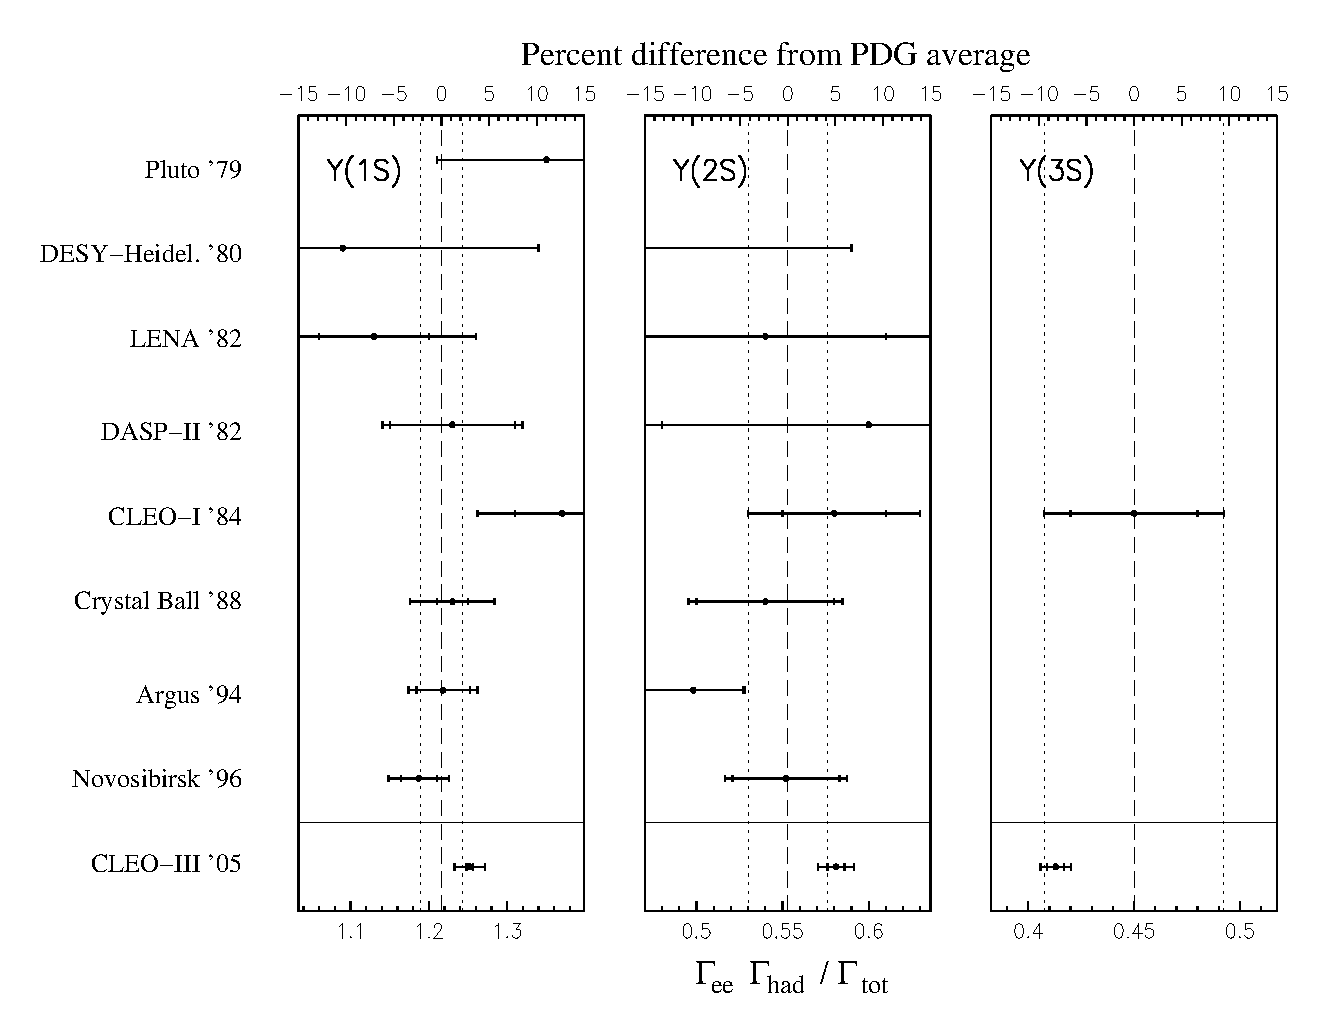
\includegraphics[width=0.9\linewidth]{pdgplots2}
  \end{center}
\end{slide}

\begin{slide}[Comparison with Theory]
  Theoretical calculation of $\Gamma_{ee}(2S)/\Gamma_{ee}(1S)$ (hep-lat:0507013, 13 July 2005)

  \vfill
  \begin{center}
    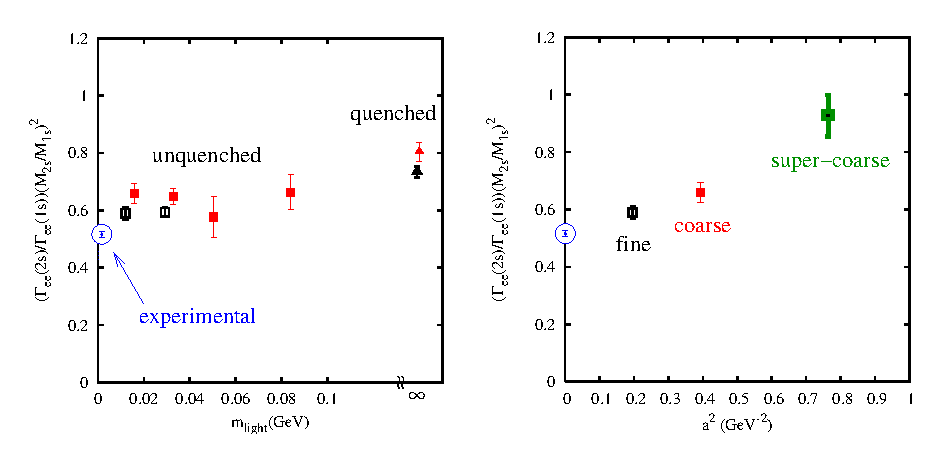
\includegraphics[width=\linewidth]{dependence}
  \end{center}

  \vfill
  Strong dependence on lattice spacing ($\Gamma_{ee} \propto |\psi(0)|^2$, one point on the lattice)

  \vfill
%  ``Fine,'' unquenched result: 0.52 $\pm$ 0.02
  ``Fine'' unquenched result: (13 $\pm$ 5)\% higher than experiment.

\end{slide}

\end{document}
